%%
%  ******************************************************************************
%  * #file    Szablon_raportu_EN_Latex.tex
%  * #author  Adrian Wójcik   adrian.wojcik(at)put.poznan.pl
%  *          
%  * #commit  Patryk Kościk   koscikpatryk(at)gmail.com
%  *          Modified the template for Projekt przejsciowy purposes          
%  *          
%  * #version 1.0
%  * #date    09-Mar-2022
%  * #brief   PROJPRZEJ
%  *
%  ******************************************************************************
%%  
\documentclass[11pt, a4paper]{article}

\usepackage{SM_template}

% Wypełnijcie te dyrektywy zgodnie z waszym tematem
% \lab      -> NAZWA CZUJNIKA, np.: 'DHT22'
% \comment  -> Króciutki opis co to, np.: 'Cyfrowy budżetowy czujnik temperatury'
%

\lab{Moduł czytnika kart SD}
\comment{Dedykowany do sterowników drukarek DS RAMPS 1.4}
\author{Dawid Wasung}
\addbibresource{bib/KY-018.bib}

% Absolutny zakaz dotykania tego tutaj bo jak dotkiecie to coś jebnie
\university{Politechnika Poznańska}
\faculty{Wydział Automatyki, Robotyki i Elektrotechniki}
\institute{Instytut Robotyki i Inteligencji Maszynowej}
\department{Zakład Sterowania i Elektroniki Przemysłowej}

\nocite{*}


%%
%
% Początek dokumentu
%
%%
\begin{document}

%% Strona tytułowa %%
\mainpage{{KY-018/foto}}
\newpage

\section*{Opis elementu} \addcontentsline{toc}{section}{Wstęp}
Moduł czytnika kart SD umożliwia odczytywanie kart MicroSD, dedykowany jest to sterowników drukarek 3D RAMPS 1.4, jest jednak wstecznie kompatybilny do wersji 1.3. Ważną cechą samego modułu jest możliwość współpracy z innymi mikrokontrolerami. Przyjmuje napięcie od 4.5V do 5.5V, transfer osiąga prędkość do 50Mb/s i osbługiwany jest po interfejsie SPI.
\vspace{0.5cm}
\begin{figure}[h!]
\centering
\begin{subfigure}{.5\textwidth}
  \centering
  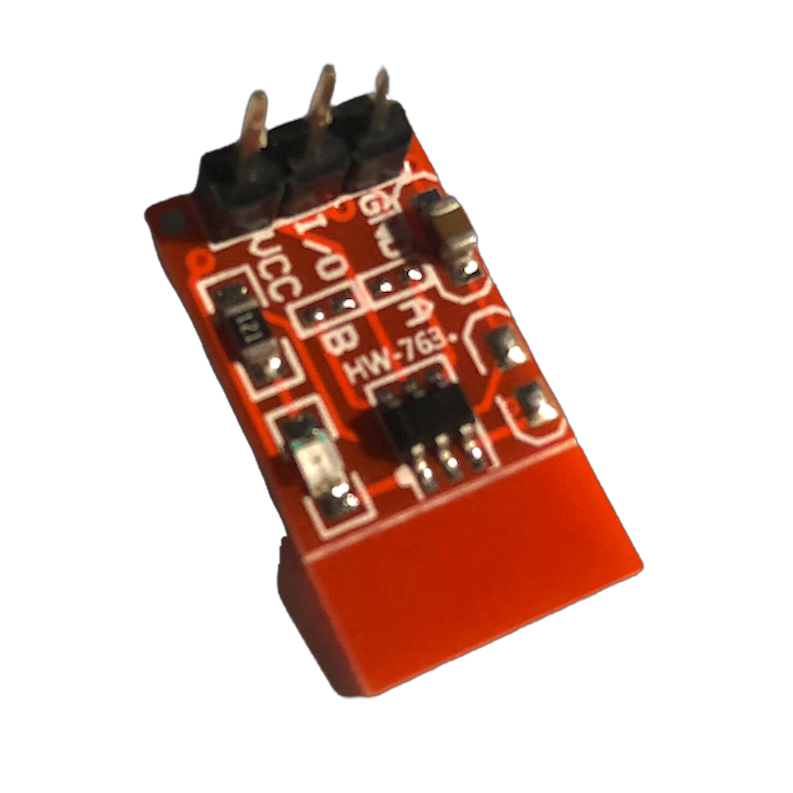
\includegraphics[width=.72\linewidth]{fig/KY-018/zdj_modułu/front.png}
  \caption{Moduł czytnika kart SD - przód}
  \label{fig:sub1}
\end{subfigure}%
\begin{subfigure}{.5\textwidth}
  \centering
  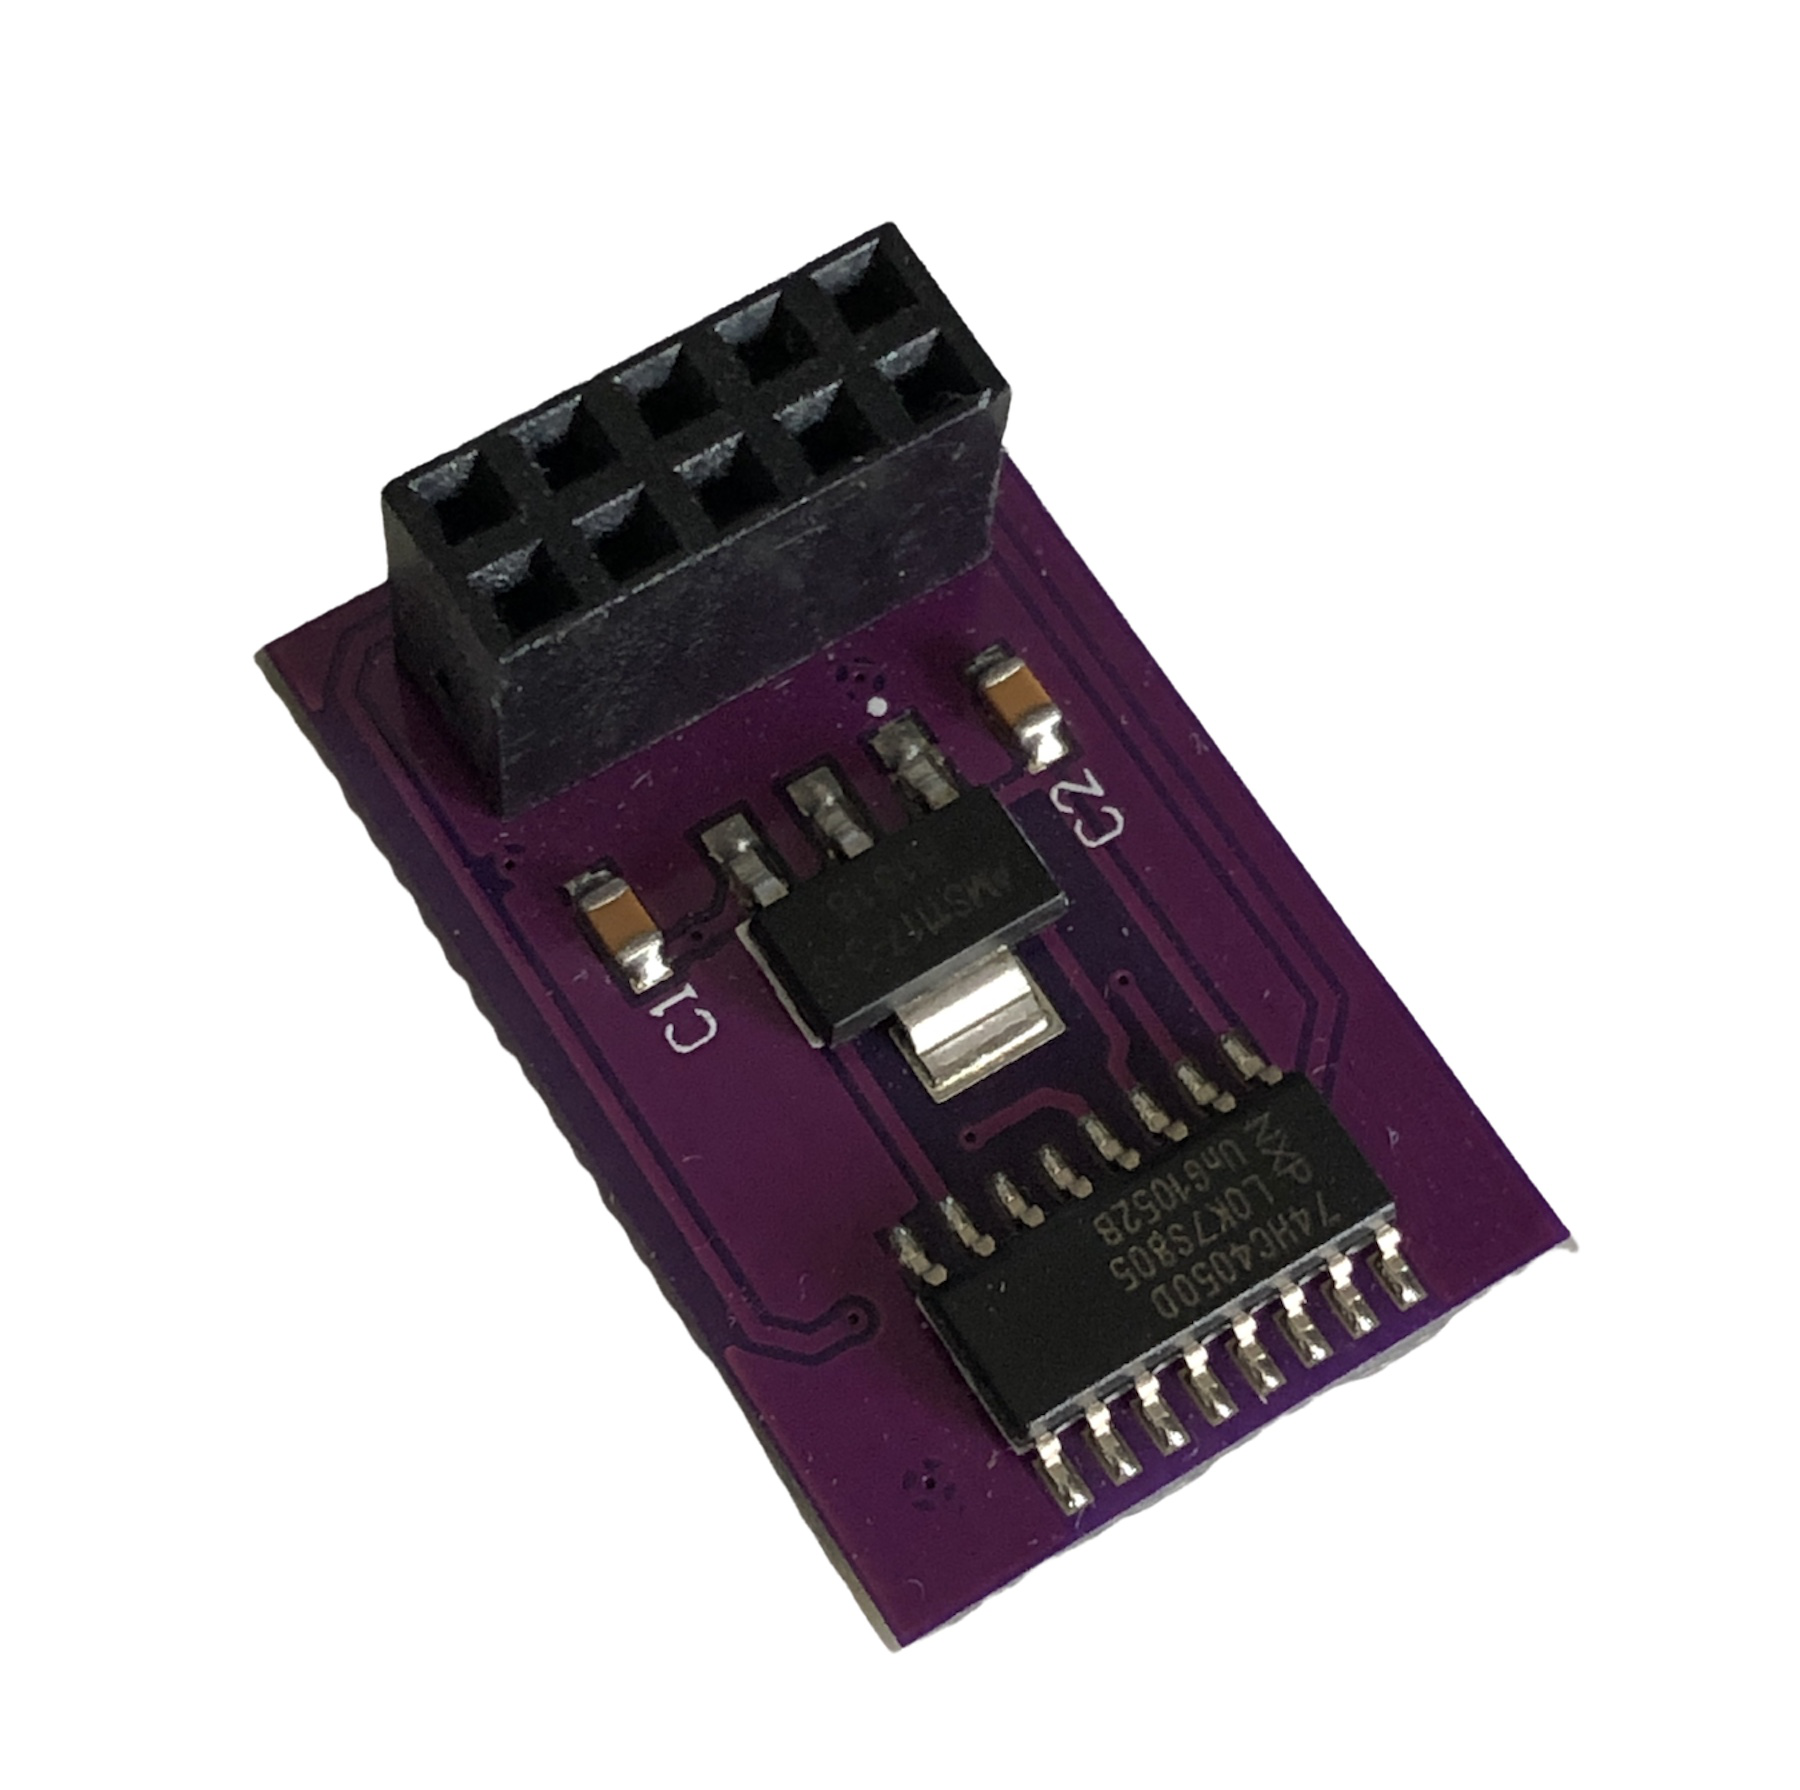
\includegraphics[width=0.748\linewidth]{fig/KY-018/zdj_modułu/back.png}
  \caption{Moduł czytnika kart SD - tył}
  \label{fig:sub2}
\end{subfigure}
\caption{Moduł czytnika kart - zdjęcia poglądowe}
\label{fig:test}
\end{figure}

Sam moduł składa się z socketu na karty MicroSD oraz dwóch komponentów - stabilizatora napięcia 1117 do 3.3V i konwertera poziomów logicznych. Napięcie robocze kart SD wynosi mniej więcej 3.3V, w związku z tym nie można jej podłączyć do układu zasilanego wyższym napięciem - przekroczenie wartości 3.6V permanentnie uszkodzi pamięć, stąd w module zamontowano stabilizator. Konwerter natomiast dopasowuje poziomy napięciowe, co jest kluczowe do współpracy z róznymi systemami i zezwala na dwukierunkową komunikację w protokole SPI w trybie full duplex.

\begin{figure}[h!]
\centering
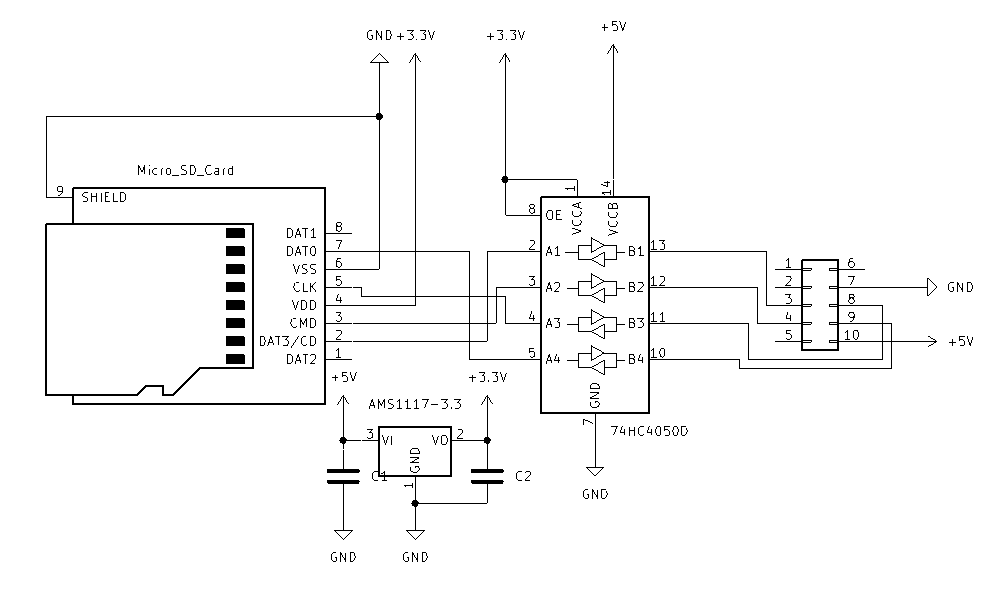
\includegraphics[width=0.81\linewidth]{fig/KY-018/zasada_dzialania/schemat2.png}
\caption{Schemat modułu}
\label{fig:sub2}
\end{figure}

\newpage
\section*{Użycie czujnika}
Karty pamięci wykorztysują system plików FAT (File Allocation Table), określający rozmieszczenie plików, katalogów oraz wolnej przestrzeni na nośniku danych. Sama nazwa pochodzi od najważniejszego elementu systemu - tabeli informującej o rozmieszczeniu plików na partycji. \\
System plików w urządzeniach wbudowanych można zaimplementować wykorzytując gotowe rozwiązania; system FAT jest jednym z lepiej udokumentowanych i prostych, co sprawiło, że publicznie dostępnych jest wiele darmowych narzędzi do administracji danych na nośniku danych wykorzystujących FAT. Jednym z takich narzędzi jest FatFs, który ma na celu bycie ,,pomostem''  między warstwą fizyczną, a aplikacją na mikrokontrolerze. Szczegółowe informacje o FatFs i sama dokumentacja dostępne są na stronie autora \cite{SD:FatFs}.

\vspace{0.5cm}
\begin{figure}[h!]
    \centering
    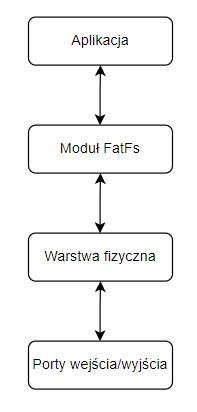
\includegraphics[width=0.18\textwidth]{fig/KY-018/działanie_ukladu/fatfs.png}
    \caption{Lokalizacja modułu FatFs w projekcie}
    \label{fig:my_label}
\end{figure}

W celu porozumiewania się mikrokontrolera z kartą SD oraz poprawnego obsługiwania systemu plików, należy odpowiednio skonfigurować interfejs SPI (master do pracy w trybie full duplex), przypisać piny i podłączyć moduł do płytki rozwojowej. 
\begin{figure}[h!]
\centering
\begin{subfigure}{.5\textwidth}
  \centering
  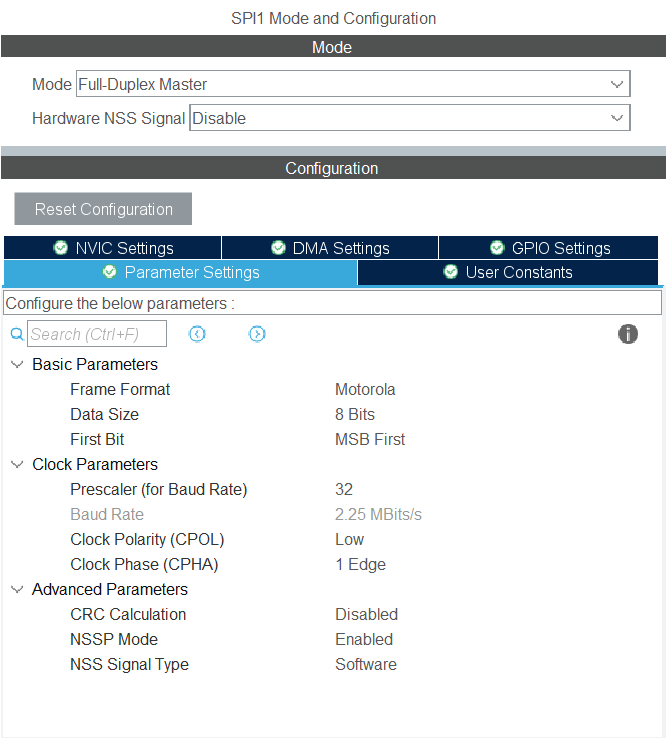
\includegraphics[width=.74\linewidth]{fig/KY-018/działanie_ukladu/spi.png}
  \caption{SPI - parametry zegara}
  \label{fig:sub1}
\end{subfigure}%
\begin{subfigure}{.5\textwidth}
  \centering
  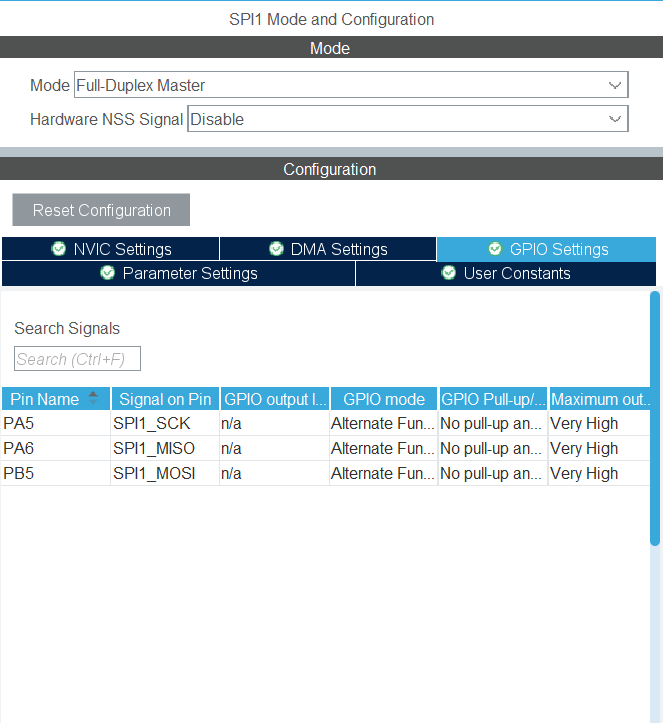
\includegraphics[width=0.74\linewidth]{fig/KY-018/działanie_ukladu/spi2.png}
  \caption{SPI - piny}
  \label{fig:sub2}
\end{subfigure}
\caption{Konfiguracja interfejsu SPI}
\label{fig:test}
\end{figure}

\newpage
\begin{figure}[h!]
\centering
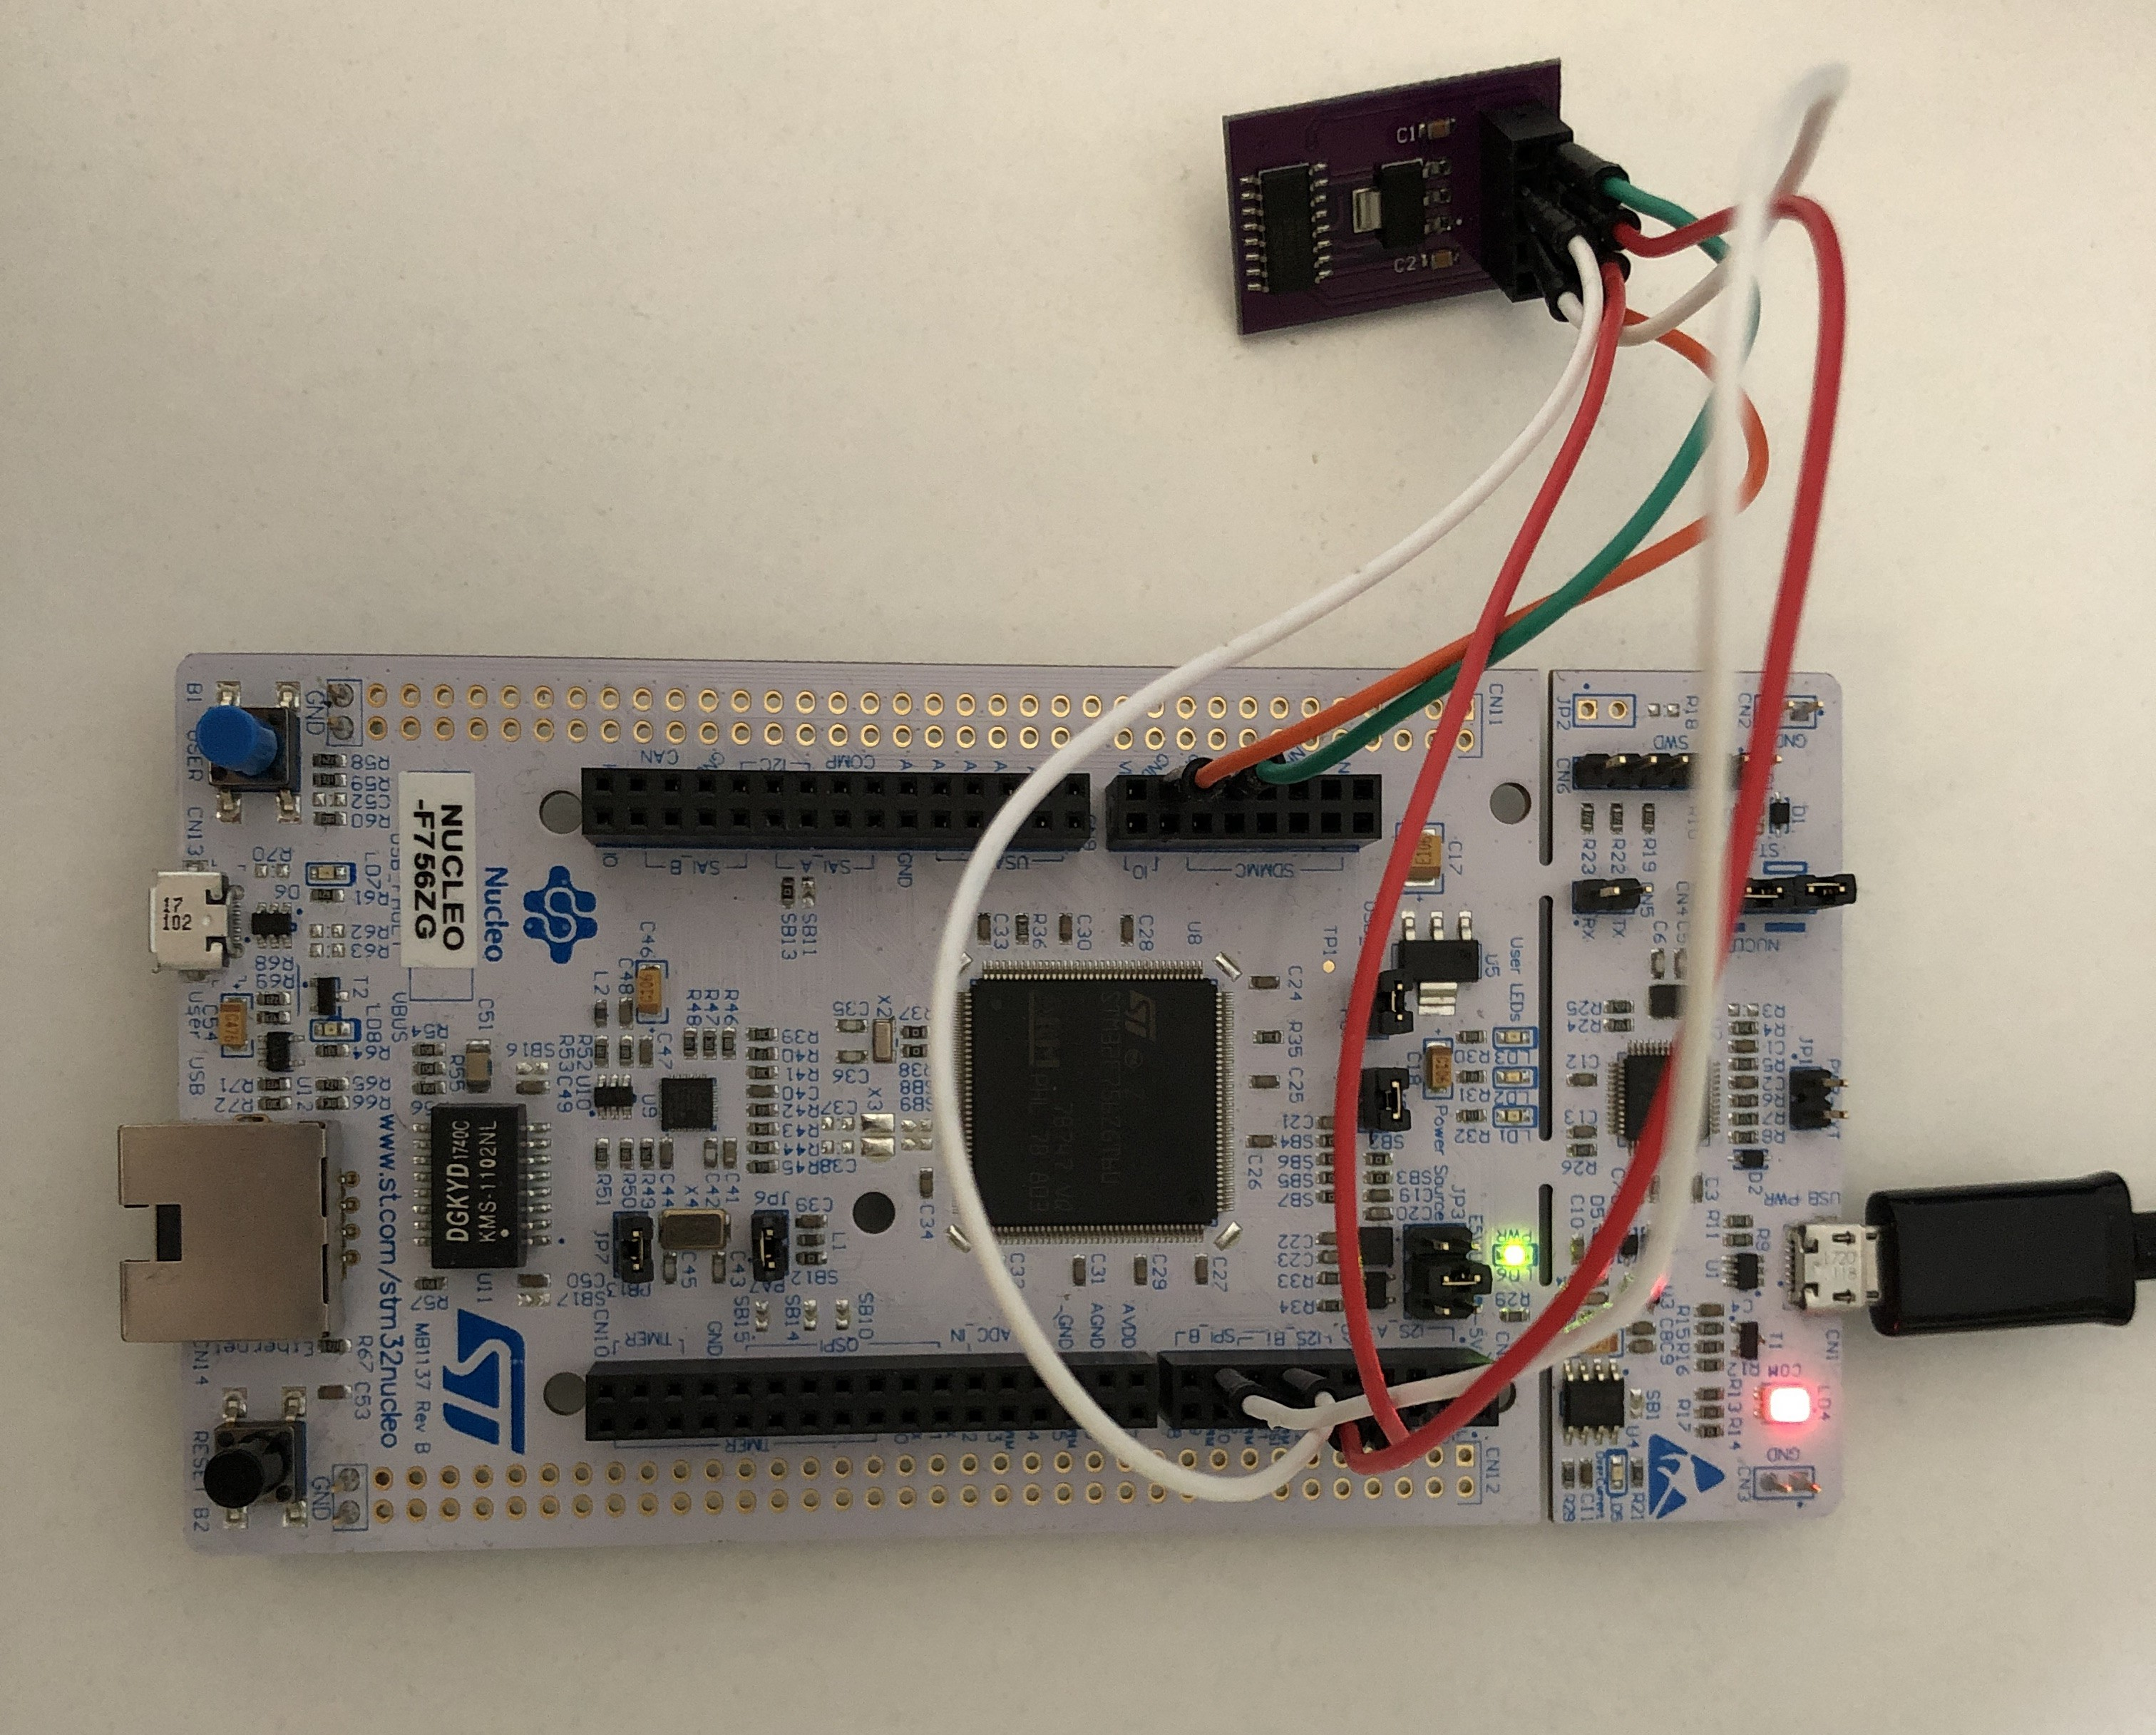
\includegraphics[width=0.7\linewidth]{fig/KY-018/polaczenie_modulu/uklad2.jpg}
\caption{Podłączony moduł}
\label{fig:sub2}
\end{figure}

Po poprawnym podłączeniu czujnika oraz konfiguracji komunikacji szeregowej SPI, można przejść do operacji na plikach i katalogach. Należy wykorzystać w tym celu predefiniowane funkcje, które oferuje moduł FatFs:
% Please add the following required packages to your document preamble:
% \usepackage{graphicx}
\begin{table}[h!]
\centering
\resizebox{\textwidth}{!}{%
\begin{tabular}{|l|l|}
\hline
\textbf{Komenda} & \multicolumn{1}{c|}{\textbf{Opis}}                                   \\ \hline
f\_mount         & Rejestracja dysku logicznego w systemie                              \\ \hline
f\_open          & Otwieranie pliku lub tworzenie, gdy go nie ma                        \\ \hline
f\_close         & Zamykanie pliku                                                      \\ \hline
f\_read          & Czytanie zawartości pliku                                            \\ \hline
f\_write         & Zapisywanie pliku                                                    \\ \hline
f\_lseek         & Przesuwa wskaźnik zapisu/odczytu pliku                               \\ \hline
f\_truncate      & Skraca długość pliku                                                 \\ \hline
f\_sync          & Działa jak f\_close, z tym, że dalej można wykonywać na nim operacje \\ \hline
f\_opendir       & Otwiera katalog                                                      \\ \hline
f\_readdir       & Czyta zawartość katalogu                                             \\ \hline
f\_getfree       & Pozwala odczytać liczbę wolnych klastrów                             \\ \hline
f\_stat          & Odczytuje informacje o pliku/katalogu                                \\ \hline
f\_mkdir         & Tworzy katalog                                                       \\ \hline
f\_unlink        & Usuwa katalog lub plik                                               \\ \hline
f\_chmod         & Zmienia atrybuty pliku lub katalogu                                  \\ \hline
f\_utime         & Zmienia datę i czas dla określonego pliku lub katalogu               \\ \hline
f\_rename        & Zmiana nazwy lub przeniesienie pliku/katalogu                        \\ \hline
f\_mkfs          & Tworzy system plików na nośniku                                      \\ \hline
f\_forward       & Czyta dane z nośnika i bezpośrednio przekazuje dalej                 \\ \hline
\end{tabular}%
}
\end{table}
\newline
Przykładowy kod pozwalający na rejestrację dysku oraz utworzenie na nim pliku tekstowego został zaprezentowany w dodatkowych materiałach, znajdujących się na końcu rozdziału. \\

Po przejściu wszystkich kroków konfiguracyjnych, zapoznaniu się z dokumentacją FatFs i napisaniu instrukcji w języku C, moduł czytnika kart SD nie powinień sprawiać kłopotów z działaniem. 
\begin{figure}[h!]
\centering
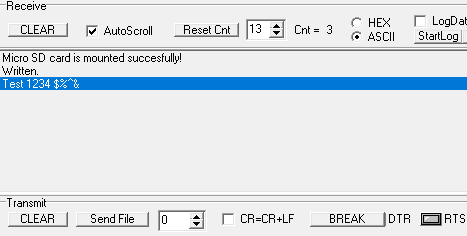
\includegraphics[width=1\linewidth]{fig/KY-018/działanie_ukladu/terminal.png}
\caption{Podłączony moduł}
\label{fig:sub2}
\end{figure}
\newline
W celu prezentacji działania modułu, do programu dodaną funkcję komunikacji szeregowej i wyświetlanie informacji w terminalu. Na Rys. 6. zaprezentowany został feedback zwrócony w terminalu podczas procesu rejestracji karty pamięci, tworzenia pliku tekstowego z zawartością oraz tekst wewnątrz pliku - wykorzystanie kodu z materiałów dodatkowych.
\begin{figure}[h!]
\centering
\begin{subfigure}{.5\textwidth}
  \centering
  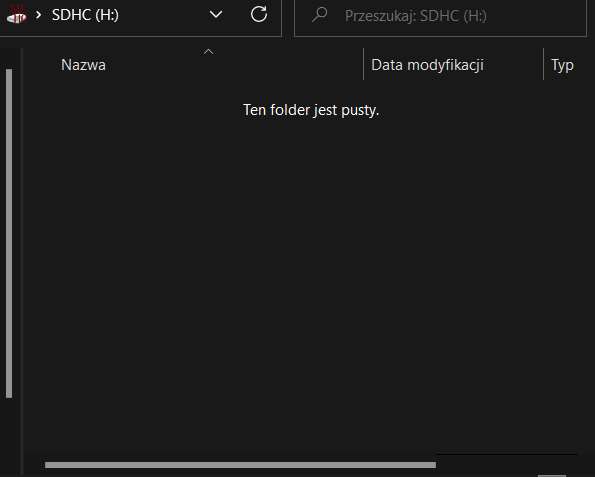
\includegraphics[width=1\linewidth]{fig/KY-018/działanie_ukladu/przed.png}
  \caption{Pusta karta pamięci przed wysłaniem instrukcji}
  \label{fig:sub1}
\end{subfigure}%
\begin{subfigure}{.5\textwidth}
  \centering
  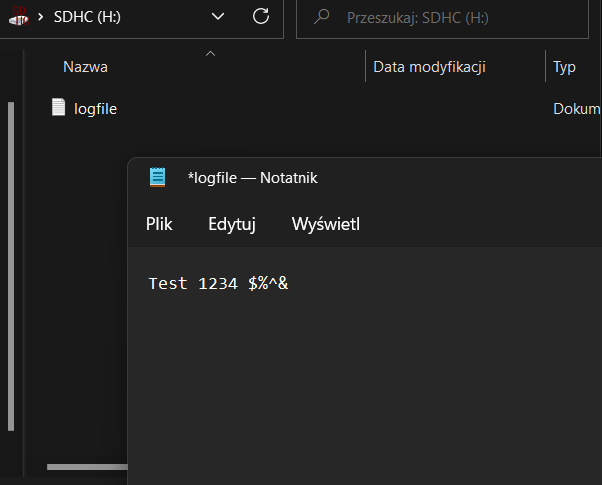
\includegraphics[width=1\linewidth]{fig/KY-018/działanie_ukladu/po.png}
  \caption{Utworzony plik tekstowy za pomocą instrukcji}
  \label{fig:sub2}
\end{subfigure}
\caption{Zawartość karty SD przed i po uruchomieniu aplikacji}
\label{fig:test}
\end{figure}
\newpage
\printbibliography[heading=bibintoc]

\end{document}